\documentclass[crop,tikz]{standalone}% 'crop' is the default for v1.0, before it was 'preview'
%\usetikzlibrary{...}% tikz package already loaded by 'tikz' option
\begin{document}
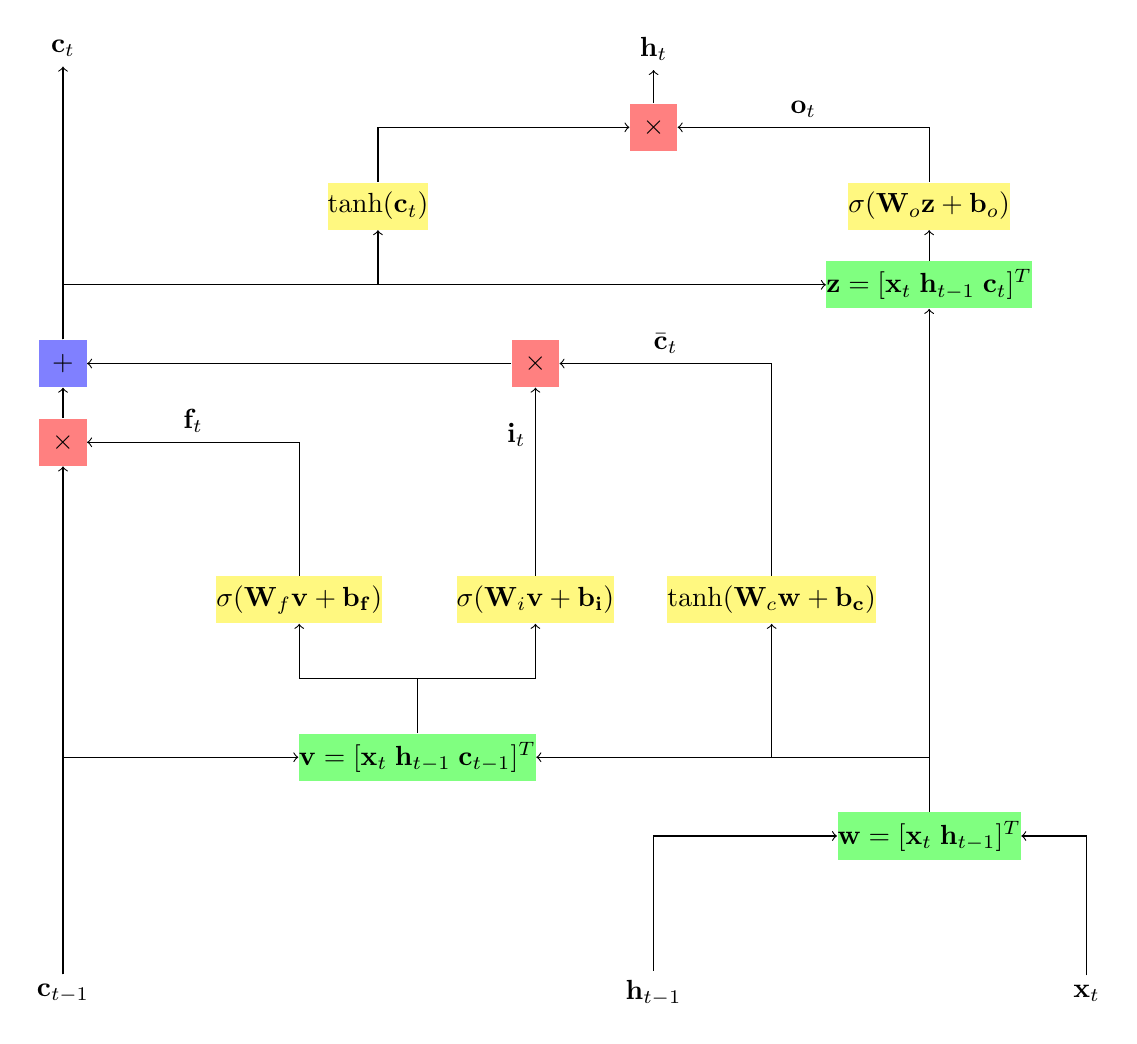
\begin{tikzpicture}
\tikzstyle{fun}=[rectangle,fill=yellow!50,minimum size=17pt,inner sep=0pt]
\tikzstyle{merge}=[rectangle,fill=green!50,minimum size=17pt,inner sep=0pt]
\tikzstyle{times}=[rectangle,fill=red!50,minimum size=17pt,inner sep=0pt]
\tikzstyle{plus}=[rectangle,fill=blue!50,minimum size=17pt,inner sep=0pt]

\node (cOld) at (0,0) {$\mathbf{c}_{t-1}$};
\node (x)    at (13,0) {$\mathbf{x}_t$};
\node (hOld) at (7.5,0) {$\mathbf{h}_{t-1}$};


\node[merge] (mergeW) at (11,2) {$\mathbf{w} = [\mathbf{x}_t \; \mathbf{h}_{t-1}]^T$};
\draw[->] (x) |- (mergeW);
\draw[->] (hOld) |- (mergeW);

\node[merge] (mergeV) at(4.5,3) {$\mathbf{v} = [\mathbf{x}_t \; \mathbf{h}_{t-1} \; \mathbf{c}_{t-1}]^T$};
\draw[->] (cOld) -- (0,3) -- (mergeV);
\draw[->] (mergeW) |- (mergeV);

\node[fun] (fSig) at (3,5) {$\sigma(\mathbf{W}_f \mathbf{v} + \mathbf{b_f})$};
\node[fun] (iSig) at (6,5) {$\sigma(\mathbf{W}_i \mathbf{v} + \mathbf{b_i})$};
\node[fun] (ctBar) at (9,5) {$\tanh(\mathbf{W}_c \mathbf{w} + \mathbf{b_c})$};

\draw[->] (mergeV) -- (4.5,4) -- (3,4) -- (fSig);
\draw[->] (mergeV) -- (4.5,4) -- (6,4) -- (iSig);
\draw[->] (mergeW) -- (11,3) --  (9,3) -- (ctBar);

\node[times] (ftimesCOld) at (0,7) {$\times$};
\draw[->] (cOld) -- (0,3) -- (ftimesCOld);
\draw[->] (fSig) |- (ftimesCOld) node[near end, above] {$\mathbf{f}_t$};

\node[times] (ctBarTimesIt) at (6,8) {$\times$};
\draw[->] (iSig) -- (ctBarTimesIt) node[near end, left] {$\mathbf{i}_t$};
\draw[->] (ctBar) |- (ctBarTimesIt) node[near end, above] {$\bar{\mathbf{c}}_t$};

\node[plus] (compCt) at (0,8) {$+$};
\draw[->] (ftimesCOld) -- (compCt);
\draw[->] (ctBarTimesIt) -- (compCt);

\node (ct) at (0,12) {$\mathbf{c}_t$};
\draw[->] (compCt) -- (ct);


\node[merge] (mergeZ) at (11,9) {$\mathbf{z} = [\mathbf{x}_t \; \mathbf{h}_{t-1} \; \mathbf{c}_{t}]^T$};

%draw the stateTanh and its connecting arrow
\node[fun] (stateTanh) at (4,10) {$\tanh(\mathbf{c}_t)$};
\draw[->] (compCt) -- (0,9) -- (4,9) -- (stateTanh);


\node[fun] (outSigTanh) at (11,10) {$\sigma(\mathbf{W}_o \mathbf{z} + \mathbf{b}_o)$};
\draw[->] (mergeW) -- (11,3) -- (mergeZ);
\draw[->] (mergeZ) -- (outSigTanh);
\draw[->] (compCt) -- (0,9) -- (4,9) -- (mergeZ);

\node[times] (compHt) at (7.5,11) {$\times$};
\draw[->] (stateTanh) |- (compHt);
\draw[->] (outSigTanh) |- (compHt) node[near end, above] {$\mathbf{o}_t$};

\node (ht) at(7.5,12) {$\mathbf{h}_t$};
\draw[->] (compHt) -- (ht);

\end{tikzpicture}
\end{document}